\documentclass[journal,12pt,twocolumn]{IEEEtran}

\usepackage{amsmath}
\usepackage{amssymb}
\usepackage{amsthm}
\usepackage{graphicx}
\usepackage{gensymb}


\parindent 0px


\vspace{3cm}
\title{ Assignment 1}

\author{\textbf{\textit{Sri Charvi}}\\
\textbf{\textit{BT21BTECH11008}}}


\begin{document}

\maketitle
\textbf{Q10(b) }: A man observes the angle of elevation of the top of the tower to be 45º.
 He walks towards it in a horizontal line through its base. On covering 20 m the angle of 
elevation changes to 60º. Find the height of the tower correct to 2 significant figures.\\

\medskip
\textbf{Solution}: Let the height of the tower be `$h$' and total distance between man and the tower be `$d$'.\\

\begin{figure}[h]
    \centering
    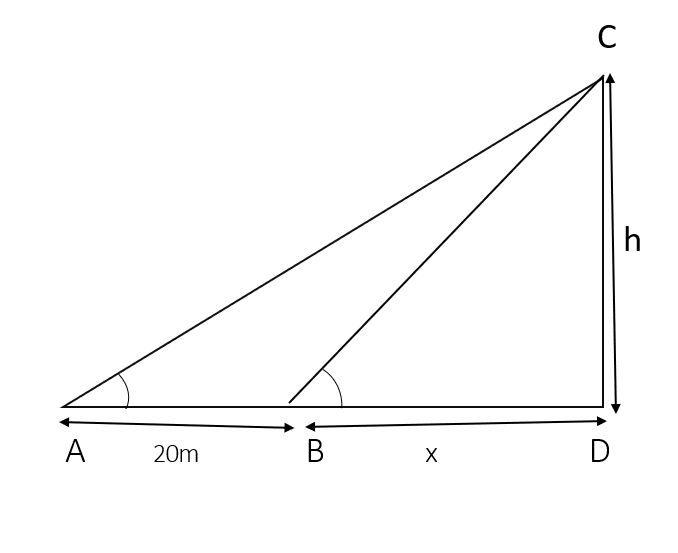
\includegraphics[width=\columnwidth]{Fig1}
    \caption{}
    \label{Fig1}
\end{figure}

 Let the given angles
be $\theta_1=45\degree \text{ and } \theta_2=60\degree.$

From the given information,
\begin{align}
\label{eq:x}
d=x_1+x_2\\
\label{eq:y}
h\cot\theta_1=d\\
\label{eq:z}
h\cot\theta_2=x_2 
\end{align}

Solving the equations \eqref{eq:x},\eqref{eq:y},\eqref{eq:z}, we get
\begin{align*}
 h\cot\theta_1&=x_1+h\cot\theta_2\\
 h&=\frac{x_1}{\cot\theta_1-\cot\theta_2}\\
 h&=\dfrac{20}{\left(1-\frac{1}{\sqrt{3}}\right)}\\
 h &= 47.32m
\end{align*}

$\therefore $ The height of the tower is 47.32 m\\


Input parameters:

\begin{table}[!h]
	\begin{tabular}{|c|c|}

   \hline
   \textbf{Variable} & \textbf{value}\\
   \hline
   $\angle CAD = \theta_1$ & $45\degree$\\
   \hline
   $\angle CBD = \theta_2$ & $60\degree$\\
   \hline
   $AB = x_1$ & $20m$\\ 
   \hline

\end{tabular}\\

   
\end{table}



\end{document}